\chapter{Related Work}
\label{cha:related-work}

Whereas the purpose of \autoref{cha:introduction} was to entice and
convince the reader that work reported is interesting, that the author
is asking the right questions about it, and reading about it will be
worthwhile, the purpose of \autoref{cha:related-work} is to
demonstrate that the author possesses a fine overview and keen
understanding of the topic of the work.  Note that while the title of
the chapter is ``Related Work'', it might as well be called
\emph{``Relevant} Work'' in that you should only include work that are
directly useful or relevant to your purpose. 

Writing about others' work can be challenging---it is easy to succumb to just
writing condensed summaries, which are just as tedious to read as they are to
write.  A better method is to gain an overview over the field of inquiry, and
then establish in the first section the aspects or dimensions that are crucial
to systems or methodologies such as the ones described. This demonstrates to
the reader that the author has understanding and judgement. Having done this,
every paper or work can then be described in those established terms. This
makes for easier and much more structured writing, and it also helps the
reader differentiate the systems and works reported on. If there are multiple
works that cover approximately the same area (\eg using the same technique),
you may mention several, but only go into detail with the most significant or
representative one.

The chapter can then be concluded with a table (see
\autoref{tab:relatedwork-summary} on \autopageref{tab:relatedwork-summary})
summarising all the work reported on using the aspects defined in the
introduction of the chapter.

One aspect to keep in mind when reading others' work is how they performed
their evaluation. This can both be a source of inspiration for your own
evaluation in \autoref{cha:evaluation}, and a point of critique, if their
evaluation is weak. It will also often be the case that different papers will
have different kinds of evaluation, making a direct comparison tricky (and
potentially something worth investigating).

A crucial element of this chapter is that it concerns the work of
others and \emph{only} that. While the selection of aspects or
dimensions described above invariantly will reflect your own focus,
that should be the extend of which your own work and plans influence
this chapter.  Your own judgement comes in the next chapter.

  \begin{sidewaysfigure}
  \centering

  \subfloat[Google Scholar.]
  {\label{fig:bibtex-1}
\includegraphics[width=.33\linewidth]{gfx/bibtex_1}}
  \subfloat[Press `"'.]
  {\label{fig:bibtex-2}
\includegraphics[width=.33\linewidth]{gfx/bibtex_2}}
  \subfloat[Press `BibTeX'.]
  {\label{fig:bibtex-3}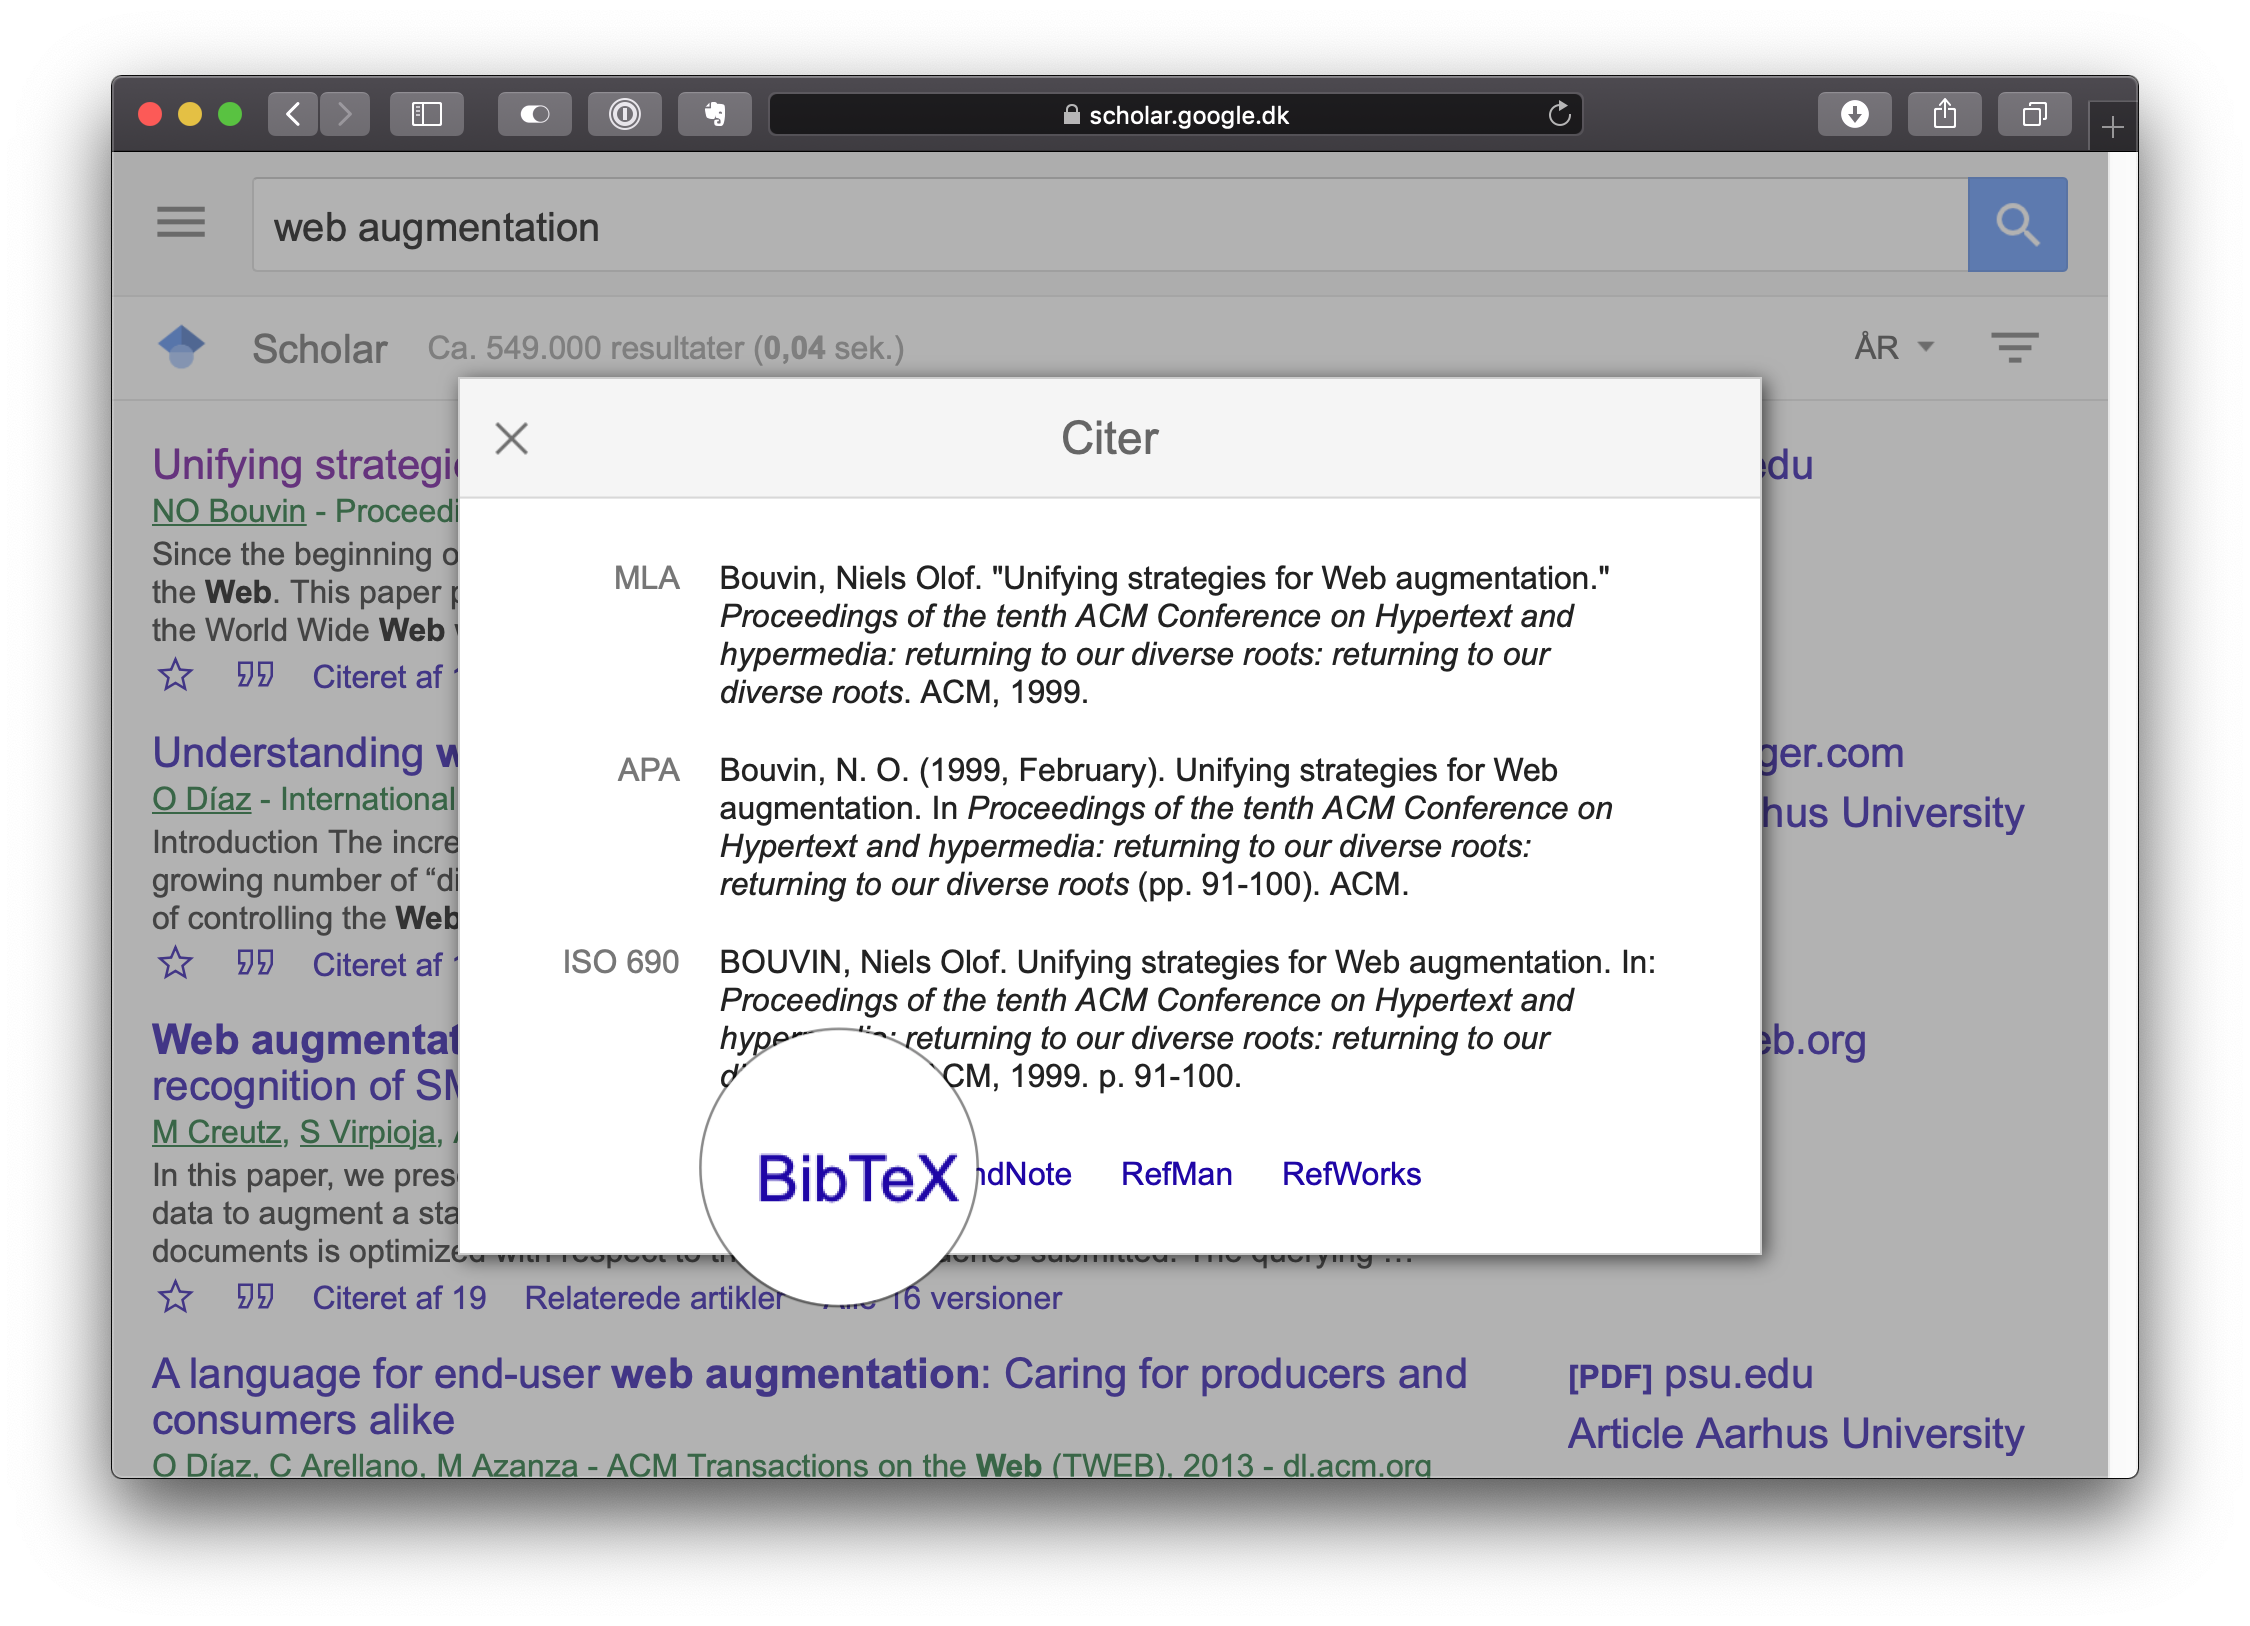
\includegraphics[width=.33\linewidth]{gfx/bibtex_3}}
  
  \subfloat[Copy the reference.]
  {\label{fig:bibtex-4}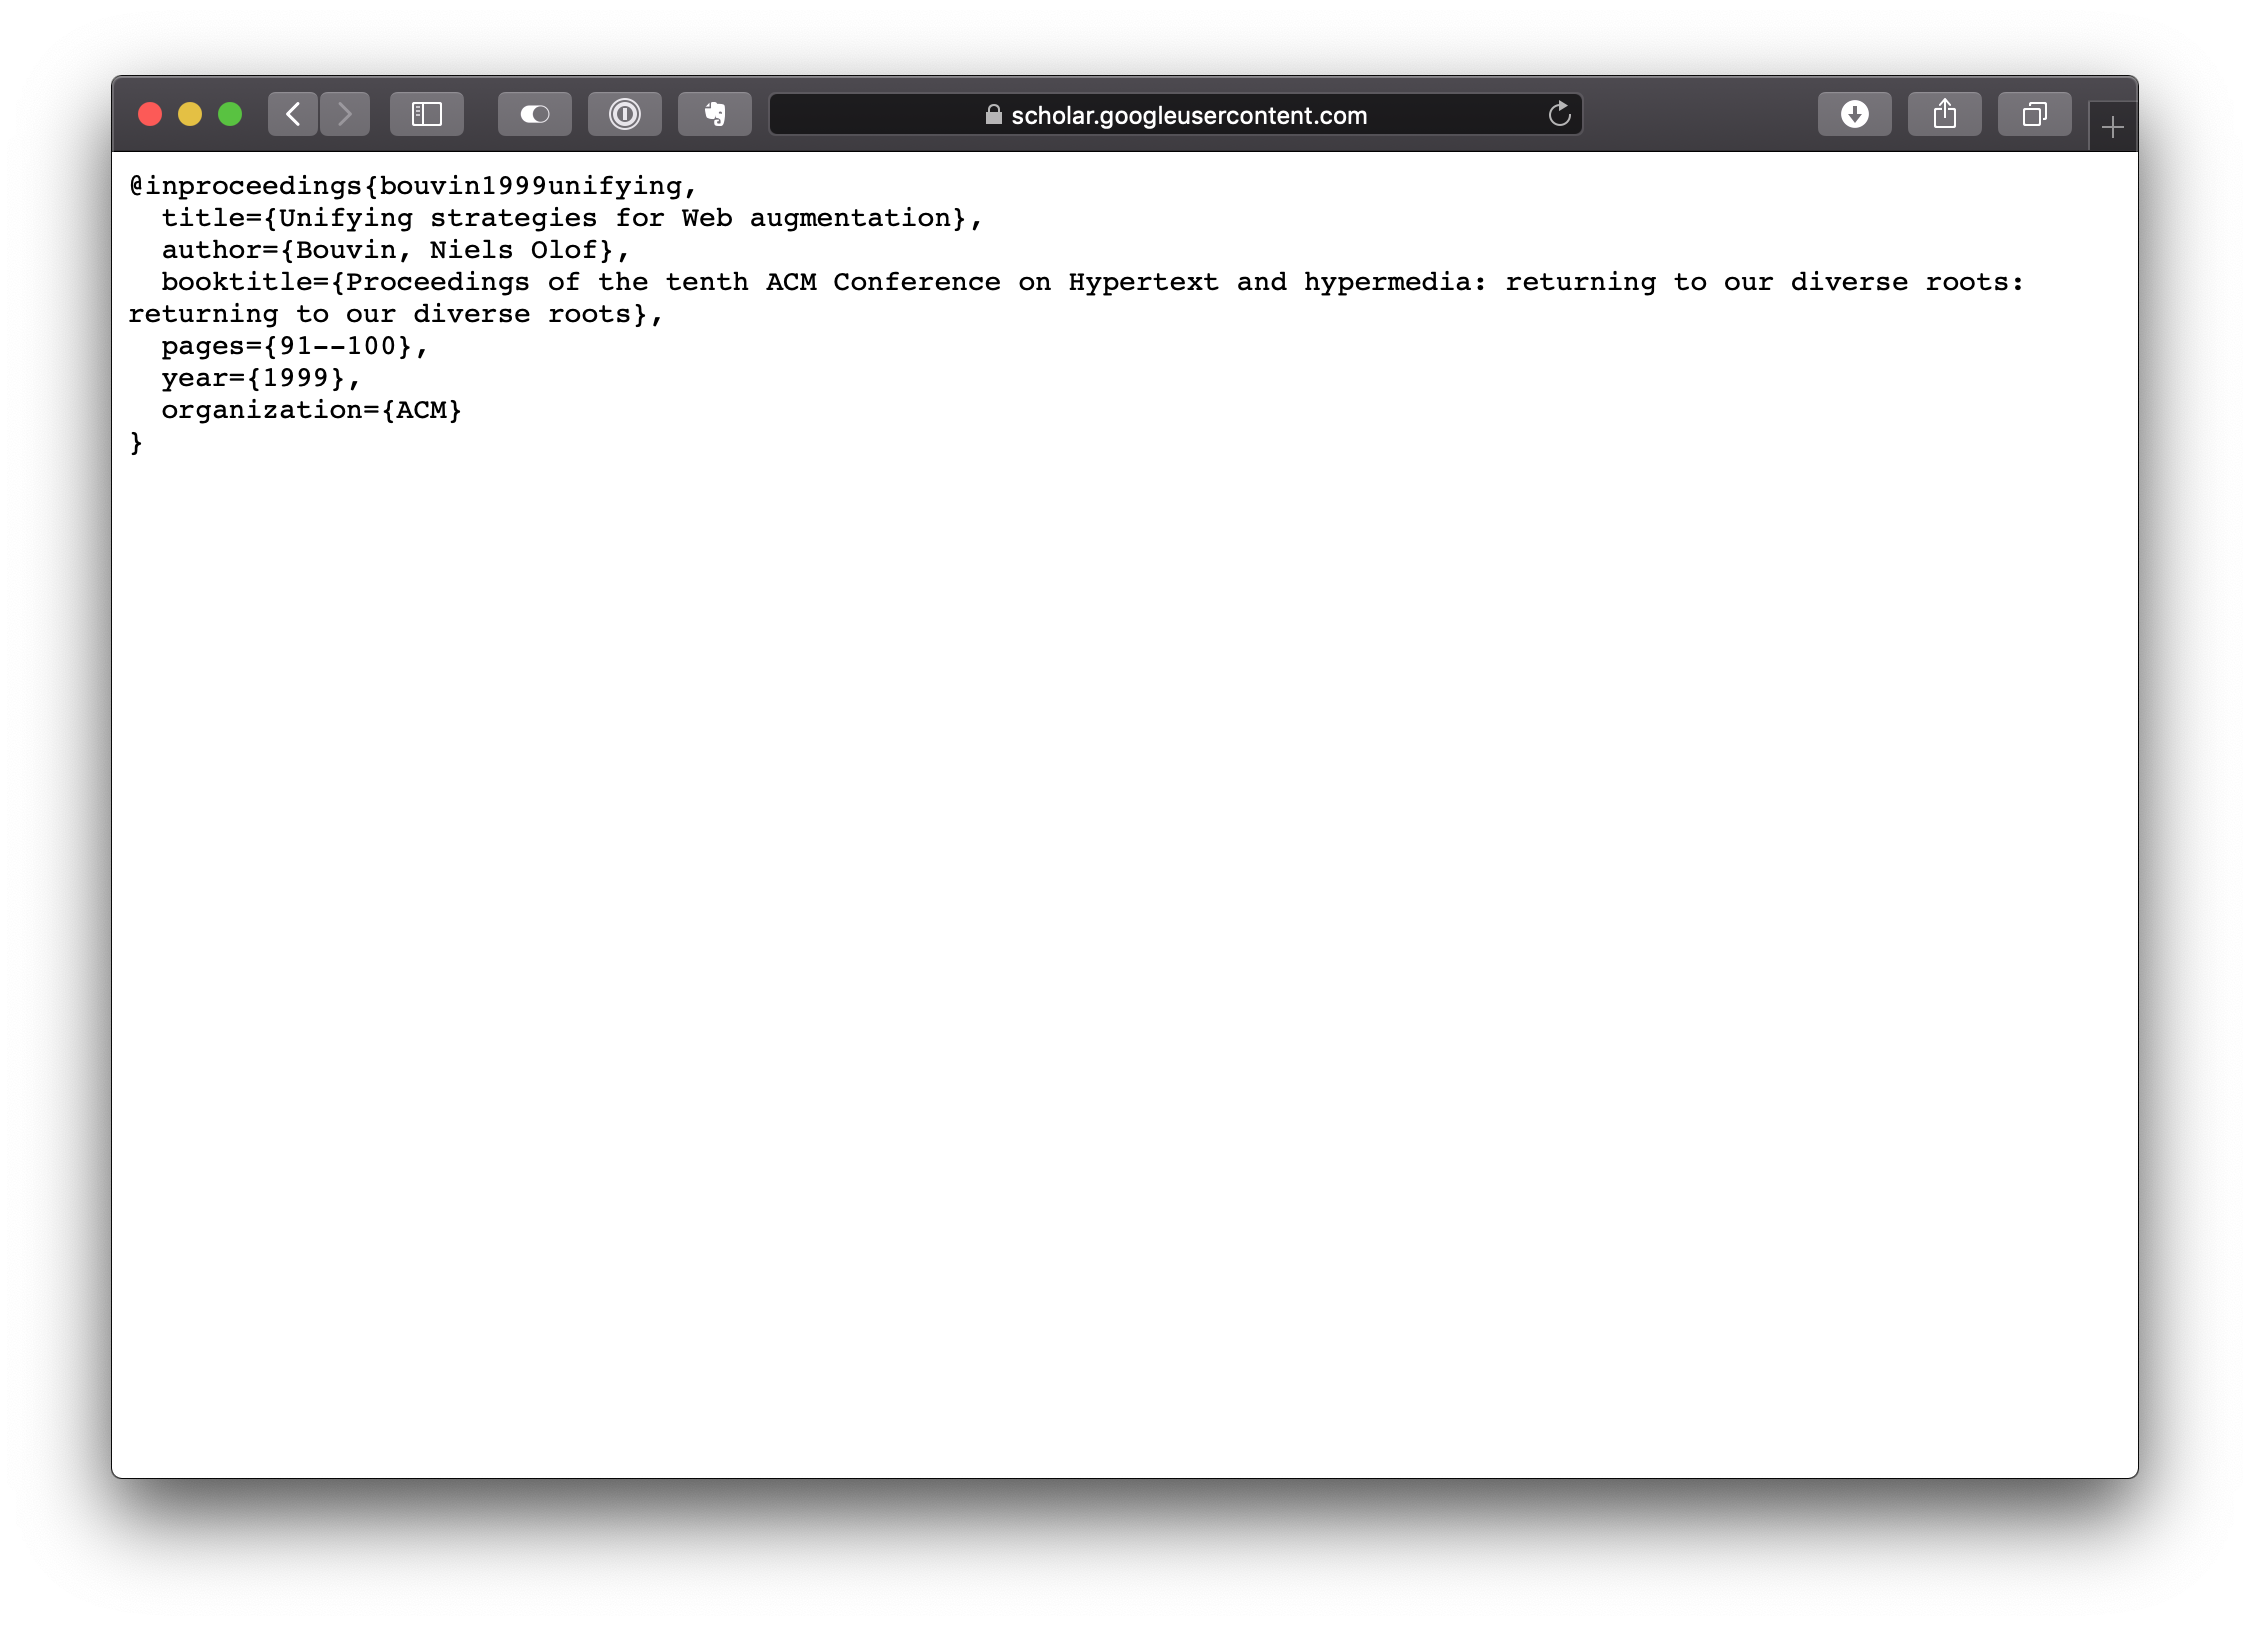
\includegraphics[width=.33\linewidth]{gfx/bibtex_4}}
  \subfloat[Follow the ACM link and press BibTeX.]
  {\label{fig:bibtex-5}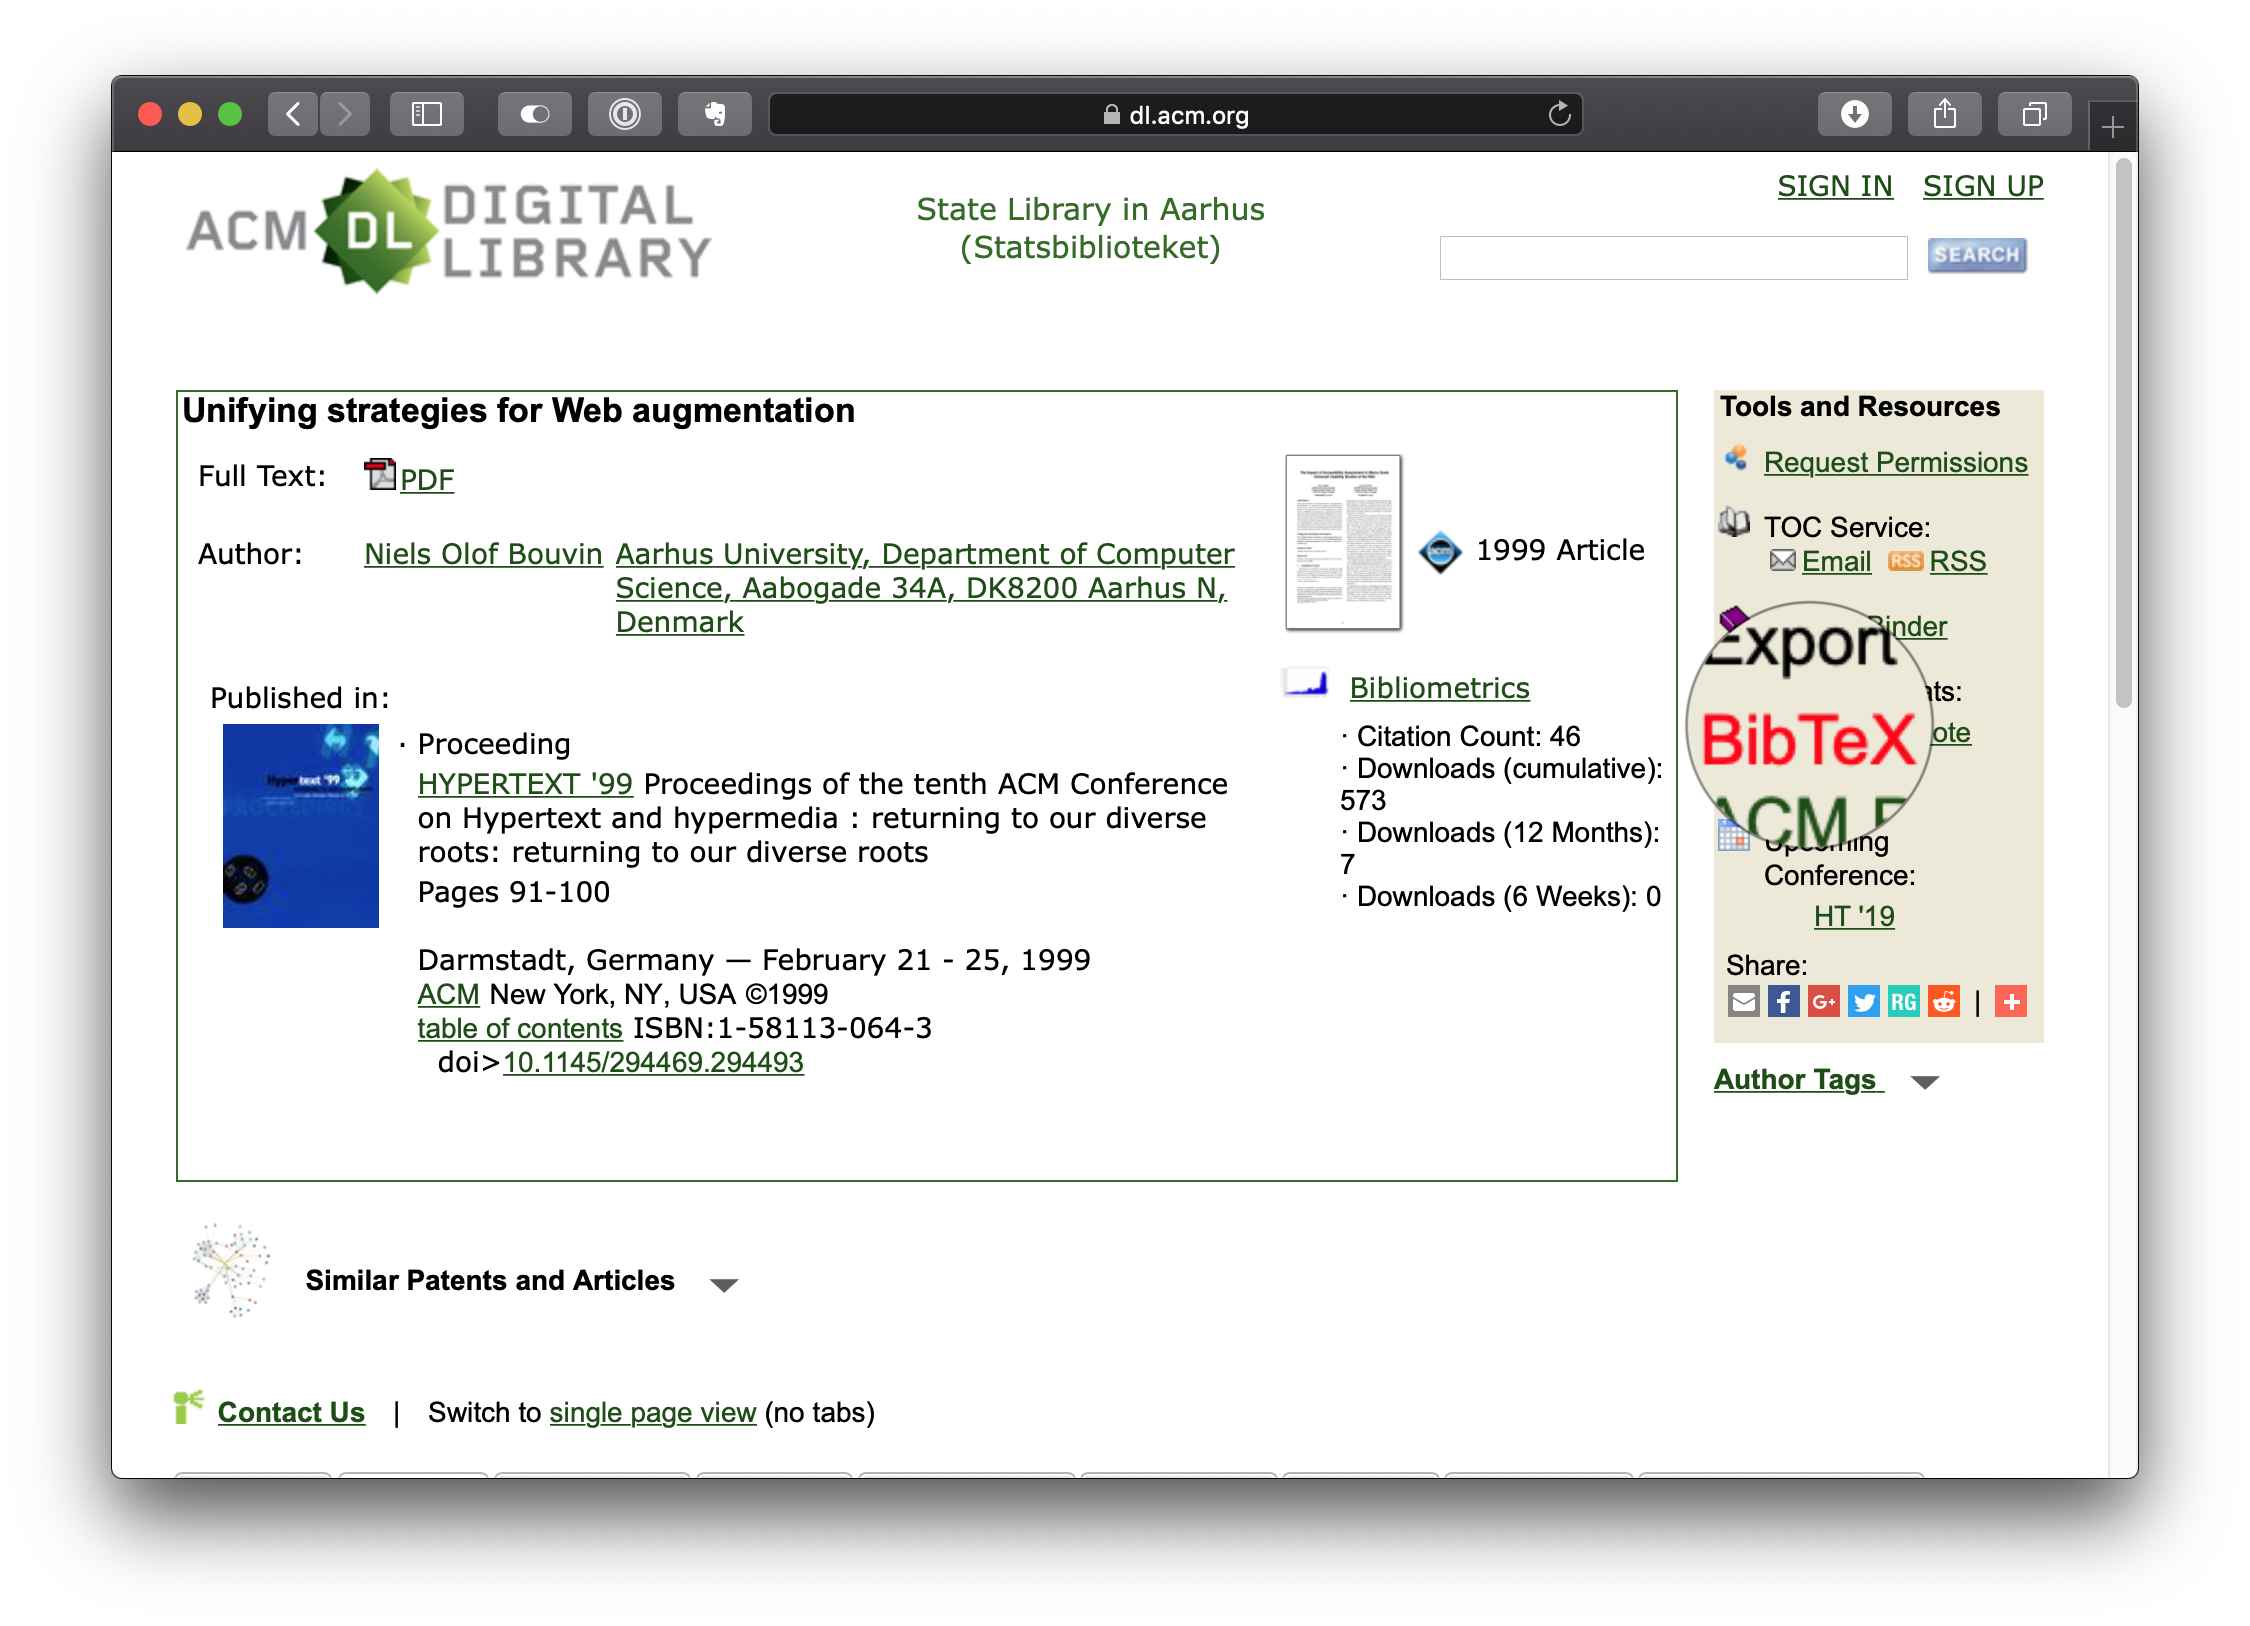
\includegraphics[width=.33\linewidth]{gfx/bibtex_5}}
  \subfloat[Copy the much better reference.]
  {\label{fig:bibtex-6}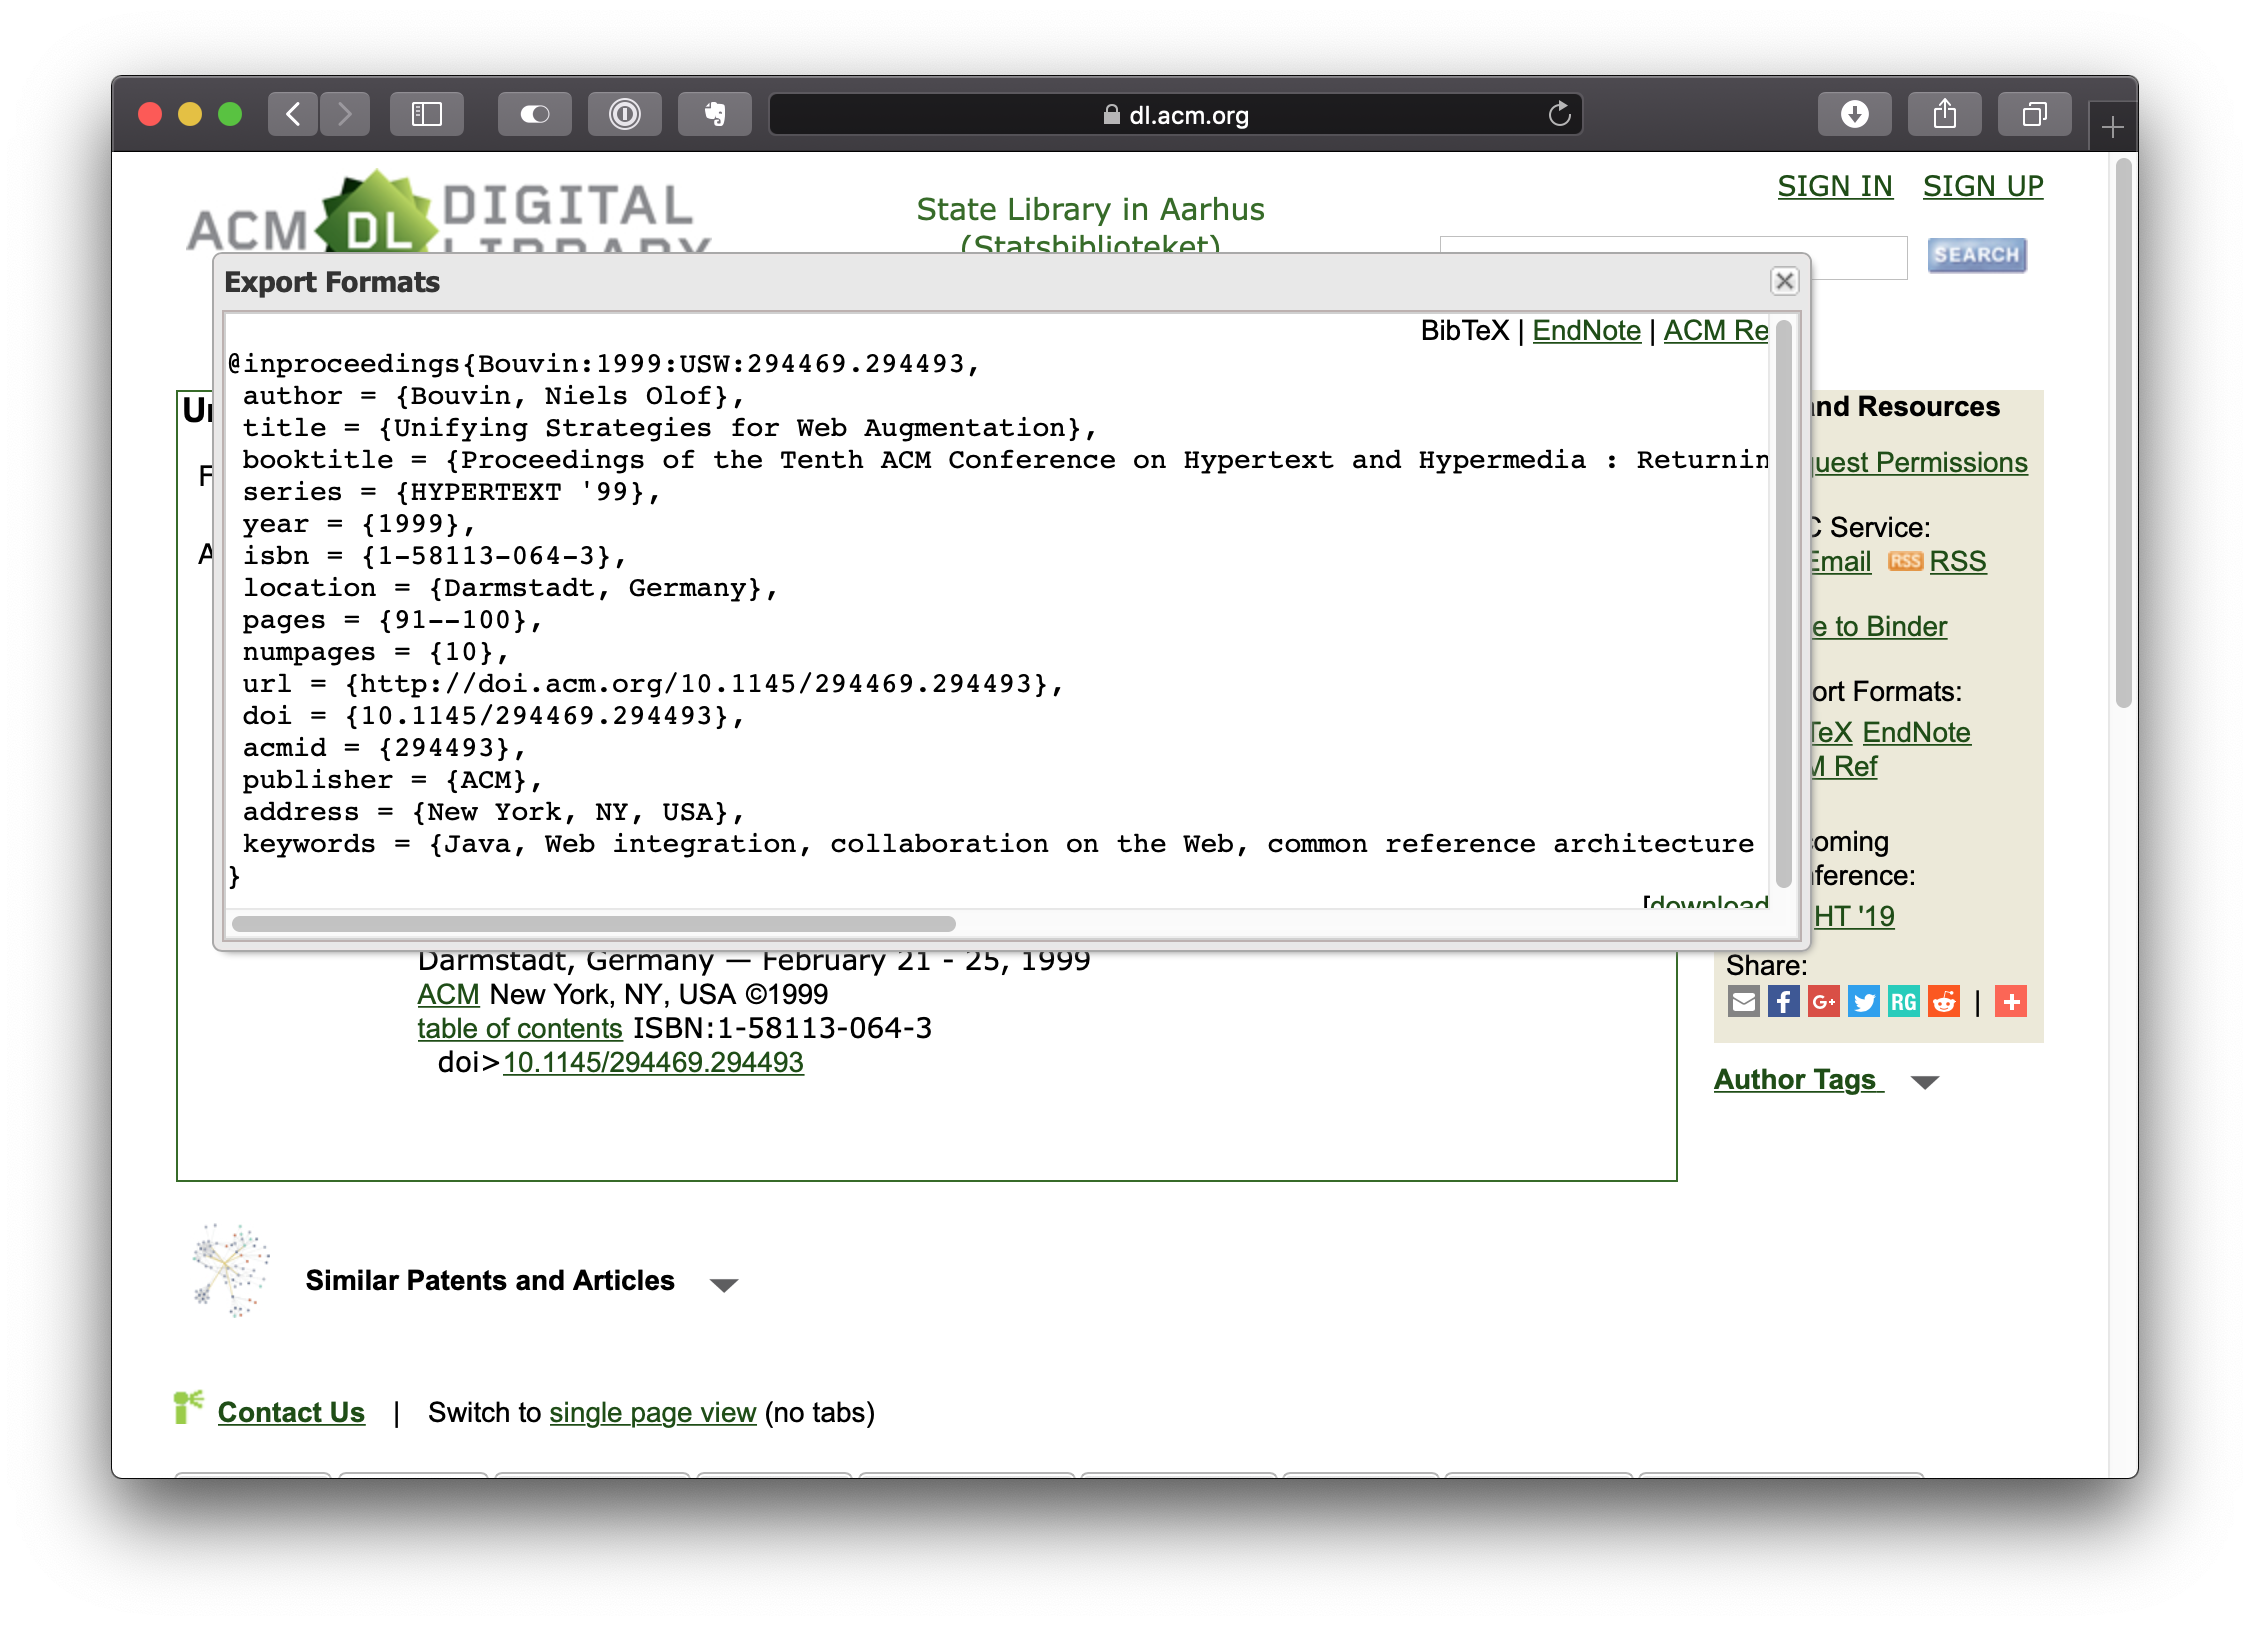
\includegraphics[width=.33\linewidth]{gfx/bibtex_6}}

  \caption[Two different ways to get good \mBibTeX\ references]{Two different ways to get good \mBibTeX\ references. The ACM method is recommended as it provides a much higher quality reference, whereas the Google Scholar reference is merely scraped.}\label{fig:bibtex}
\end{sidewaysfigure}


\section{A small note on references}
\label{sec:small-note-refer}

It is essential for any scientific work to cite its sources. This can be done
relatively painlessly using \mBibTeX\ as outlined on
\autopageref{sec:handl-bibl}. It is important that you include all necessary
information in the bibliography for others to correctly identify and locate the
referenced work, and the easiest way to do that is to copy the \mBibTeX\
reference straight from ACM, as seen in \autoref{fig:bibtex}.  Other publishers usually also have \mBibTeX\ references available. If you cite one
work, it should be done thus \cite{Kristensen2010:MP2P2010}, if you cite a
specific page in a work, it should be done thus
\cite[p. 410]{Chawathe2003:2003}, and if you cite multiple works, it should be
done thus
\cite{knuth:1976,knuth:1974,Kristensen2010:MP2P2010,Mittelbach2004:TLC2004}.  I
generally reserve the bibliography for works that have been properly published
and/or peer reviewed. References to Web pages are best handled through
footnotes\footnote{\url{https://www.tug.org/applications/pdftex/} accessed
  2018/6/27.} (or marginalia\marginpar{\scriptsize\url{http://lyx.org/}}, if they are very
short), though some things, such as
RFCs and other standard documents, belong in the bibliography proper. If you use
a figure from another work, you \emph{must} give attribution---otherwise it counts
as plagiarism, which is a serious offence.


\section{Frameworks and Technologies}
\label{sec:fram-techn}

Related work need not only be published academic work. In many cases, it is
also relevant to describe crucial frameworks and technologies that will be
used or are relevant for the thesis.  This does not mean that all employed
technologies should be described in detail, but frameworks and technologies
that are unusual (for lack of a better word) could be described here. \Eg
there is no need to describe an ordinary network stack, but if the work
involves GPU programming, a description of the chosen architecture might well
be relevant, as it informs all the following chapters.  In short, if it is
something a CS generalist should be familar with, there is no need to describe
it.

\section{Summary}
\label{sec:summary}
As described above, ending the chapter with a figure like
\autoref{tab:relatedwork-summary} summarising the findings can be a great way
to remind the reader of the results, as well as laying the foundation for
\autoref{cha:analysis}.


\begin{landscape}
  \begin{table}[h]
    \myfloatalign
    \begin{minipage}{.5\linewidth}
      \renewcommand\thefootnote{\thempfootnote}
      \begin{tabularx}{\textwidth}{Xccccc} \toprule
        \tableheadline{System} & \tableheadline{Aspect} & \tableheadline{Aspect} & \tableheadline{Aspect} & \tableheadline{Aspect} & \tableheadline{Aspect} \\ \midrule
        Foo  & Y    & (Y)  & N   & (Y) & N/A\footnote{Not Applicable}\\
        Bar  & (Y)  & Y    & (N) & N   & (Y)\footnote{Only for positive integers, and not on Thursdays}\\
        Baz  & (Y)  & N    & N/A & Y   & Y\\
        Quux & N    & (Y)  & (Y) & (Y) & Y\\
        \bottomrule
      \end{tabularx}
      \caption[Summary of systems]{The systems and papers described in \autoref{cha:related-work}. The systems have been rated along the chosen aspects. Note, how this description is very much longer than what appears in the List of Tables. Using both a short and long description is a good idea---it leaves a tidy index and provides rich information where it is needed. This table is rotated (see the source to see how)---not because it is strictly needed, but to show how it might be done with wider figures.}
      \label{tab:relatedwork-summary}
    \end{minipage}
  \end{table}
\end{landscape}


%%% Local Variables:
%%% mode: latex
%%% TeX-master: "../ClassicThesis"
%%% End:
